\newpage
\appendix

\section{Directional Distance Encoding (DDE)}
\label{appendix: dde}

\begin{figure}
    \centering
    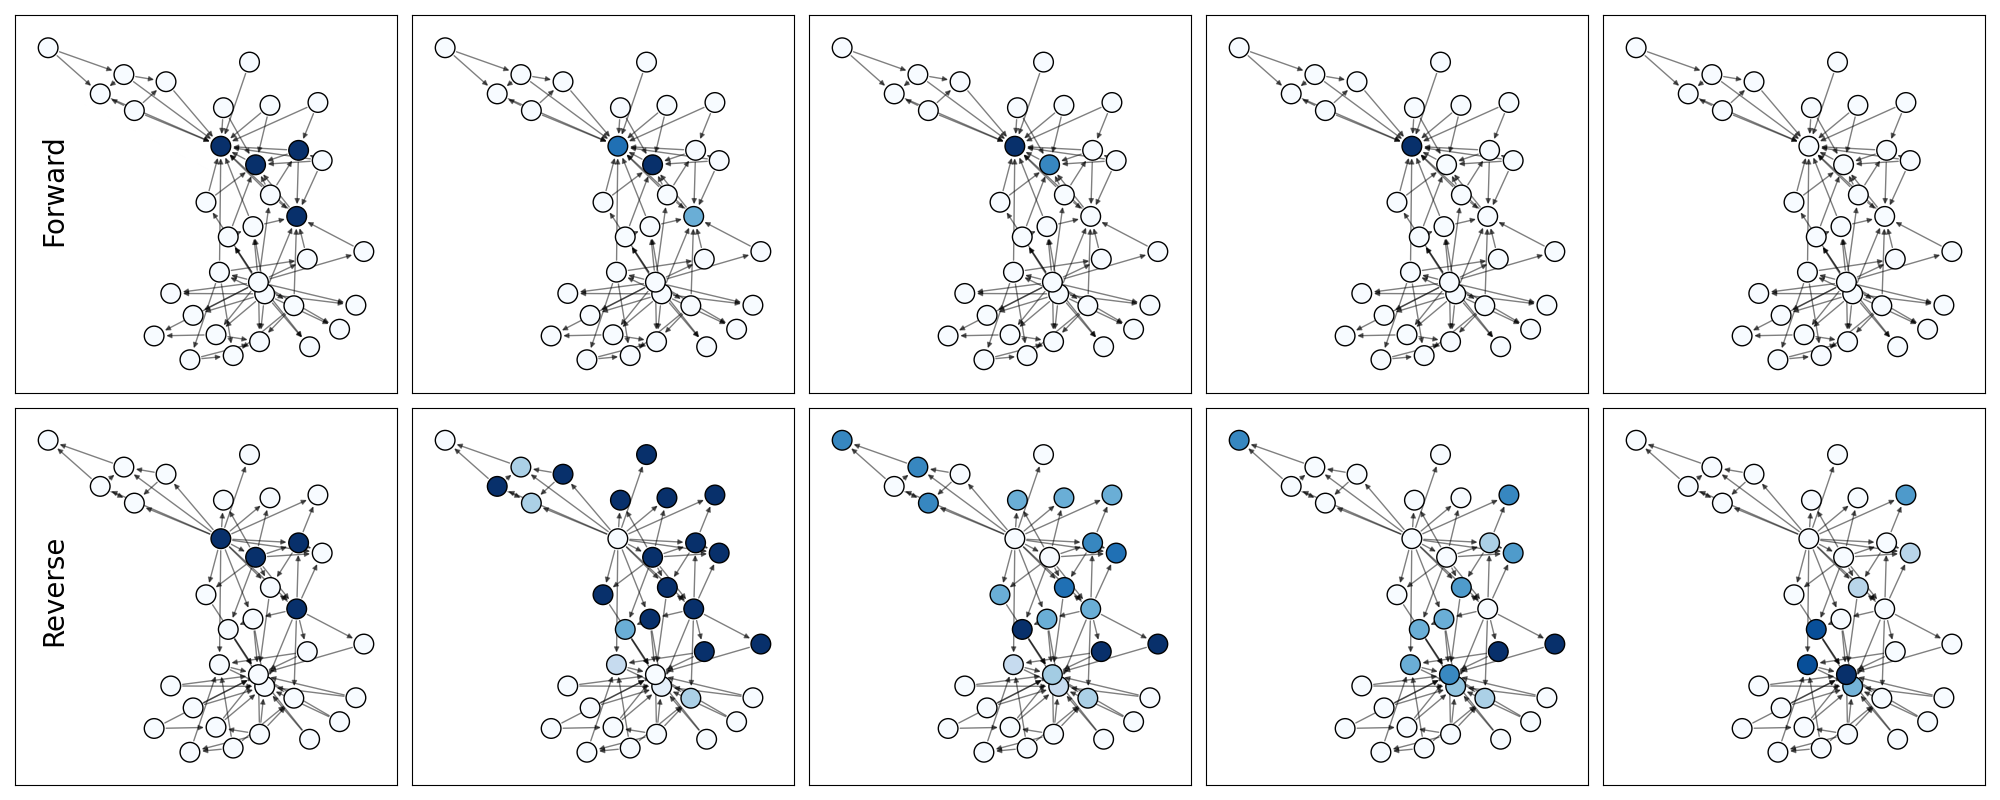
\includegraphics[width=\linewidth]{figs/DDE.png}
    \caption{A visual illustration of DDE, where the leftmost column highlights the topic entities in color. From left to right, we iteratively perform graph diffusion over the directed edges. The color intensity indicates the magnitude of the diffusion weights for individual entities.
    \label{fig:dde}}
\end{figure}

Fig.~\ref{fig:dde} provides a visual illustration of DDE. By passing entity labeling information in both directions for multiple rounds, DDE efficiently approximates measures such as the average distance between an entity and all topic entities. This process implicitly reveals information like whether an entity lies at the intersection of paths of particular lengths connecting multiple topic entities.

\section{Additional Related Work}
\label{appendix: related}

The field of KGQA has evolved significantly over time. Early approaches to KGQA do not rely on LLMs for answer generation~\citep{yasunaga2021qa,taunk2023grapeqa,zhang2022subgraph,lin2019kagnet,sun2019pullnet}, though they often employ pre-trained language models (PLMs) like BERT as text encoders~\citep{devlin-etal-2019-bert}. These methods typically search for answer entities with GNNs~\cite{yasunaga2021qa,taunk2023grapeqa,lin2019kagnet} or LSTM-based models~\cite{sun2019pullnet,zhang2022subgraph}.

With the rapid advancement of LLMs in recent years, researchers began to leverage them in KGQA. For instance, recent work has explored using LLMs as translators, converting natural language questions into executable SPARQL queries for KG databases to retrieve the answers~\citep{jiang2023structgpt,wang2023knowledgpt,luo-etal-2024-chatkbqa, xiong-etal-2024-interactive}. 

Contemporary approaches have further expanded the role of LLMs, utilizing them for both knowledge retrieval from KGs and reasoning~\citep{kim2023kg, gao2024two, wang2024knowledge, guo2024knowledgenavigator, ma2024think, sun2024think, jiang2024kg, jin2024graph}. The strength of this strategy lies in LLMs' ability to handle multi-hop tasks by breaking them down into manageable steps. However, as discussed in Section~\ref{sec:intro}, this often necessitates multiple LLM calls, resulting in high latency. To mitigate this issue, some frameworks have attempted to fine-tune LLMs to memorize knowledge, but this reduces their ability to generalize to dynamically updated or novel KGs~\citep{luo2024rog, mavromatis2024gnn}. Other models have explored fine-tuning adapters embedded in fixed LLMs to better preserve their general reasoning capabilities while adapting to specific KGs~\citep{he2024g,gao2024two,hu2024grag}.

In parallel with these developments, several approaches have emerged that, like our approach, allow LLMs to reason over subgraphs~\citep{kim2023kg,liu2024explore,li2023graph,guo2024knowledgenavigator,wu2023retrieve,li2024graph,wen2023mindmap}, though they employ different retrieval strategies. \citet{kim2023kg} breaks queries into sub-queries, retrieving evidence for each sub-query before reasoning over the collected evidence. \citet{guo2024knowledgenavigator} uses PLM-based entity extraction followed by multi-hop expansion for retrieval. \citet{li2023graph} linearizes KG triples into natural language for global triple retrieval using BM25 or dense passage retrievers. \citet{wen2023mindmap} extracts topic entities and merges triples into the retrieved subgraph using two heuristic methods: connecting topic entities via paths and retrieving their 1-hop neighbors. 

While these subgraph retrieval strategies share similarities with SubgraphRAG, they lack several key advantages of it, such as retrieval efficiency, adjustable subgraph sizes, and flexible subgraph types. Consequently, they frequently result in suboptimal coverage of relevant information in the retrieved subgraphs. SubgraphRAG addresses these limitations, offering a more comprehensive and adaptable approach to KGQA that builds upon and extends the capabilities of existing methods, while fully leveraging the power of advanced LLMs.

\section{Additional Experiment Details for Subgraph Retrieval}

\subsection{Additional Implementation and Evaluation Details}
\label{appendix:retrieval_exp_details}

For Retrieve-Rewrite-Answer, RoG, G-Retriever, GNN-RAG, and SR+NSM w E2E, we utilize their official open-source implementations for training and evaluation. While a pre-trained RoG model is publicly available, it was jointly trained on the training subset of both WebQSP and CWQ, causing a label leakage issue due to sample duplication across the two datasets. To address this, we retrain the RoG model separately on the training subset of WebQSP and CWQ. Both Retrieve-Rewrite-Answer and G-Retriever were originally only evaluated on the WebQSP dataset. We managed to adapt the G-Retriever codebase for an evaluation on the CWQ dataset. While SR+NSM w E2E originally also reports the results for CWQ, we failed in running the official codebase for this dataset.

RoG, G-Retriever, the cosine similarity baseline, GNN-RAG, and all \proj variants perform relevant subgraph retrieval from the identical rough subgraphs. These subgraphs are centered around the topic entities and are included in the released RoG implementation. In contrast, Retrieve-Rewrite-Answer directly loads and queries the raw KG.

GraphSAGE originally only deals with node attributes and we propose a straightforward extension of it for handling both the node attributes and edge attributes. Let $\textbf{z}_e$ be the text embedding of an entity $e\in \gE$ and $\textbf{z}_r$ be the text embedding of a relation $r\in \gR$. A GraphSAGE layer updates entity representations with 
\begin{align}
    & \textbf{z}_{\mathcal{N}(e)}^{l+1} = \textbf{MEAN}\left(
        \left\{
            [\textbf{z}_{e'}^{l} \|  \textbf{z}_r]      
            \mid 
            (e', r, e) \in \gG
        \right\}
    \right),
    \\
    & \textbf{z}_{e}^{l+1} = \sigma\left([\textbf{z}_{e}^{l} \|  \textbf{z}_{\mathcal{N}(e)}^{l+1}\right),
    \\
    & \textbf{z}_{e}^{0} = \textbf{z}_e,
\end{align}
where $\sigma(\cdot)$ is an MLP. Empirically, we find that 1-layer GraphSAGE yields the best performance.

\subsection{Implementation Dependencies}

Our implementation is based on the following packages: PyTorch~\citep{PyTorch}, Transformers~\citep{wolf-etal-2020-transformers}, xFormers~\citep{xFormers2022}, NetworkX~\citep{networkx}, and PyTorch Geometric~\citep{Fey/Lenssen/2019}. We employ the built-in implementation of PPR from NetworkX.

\subsection{Additional Experiment Results for Varying K in Top-K Triple Retrieval}
\label{appendix:retrieval_k}

\begin{figure*}[t]
    \centering
    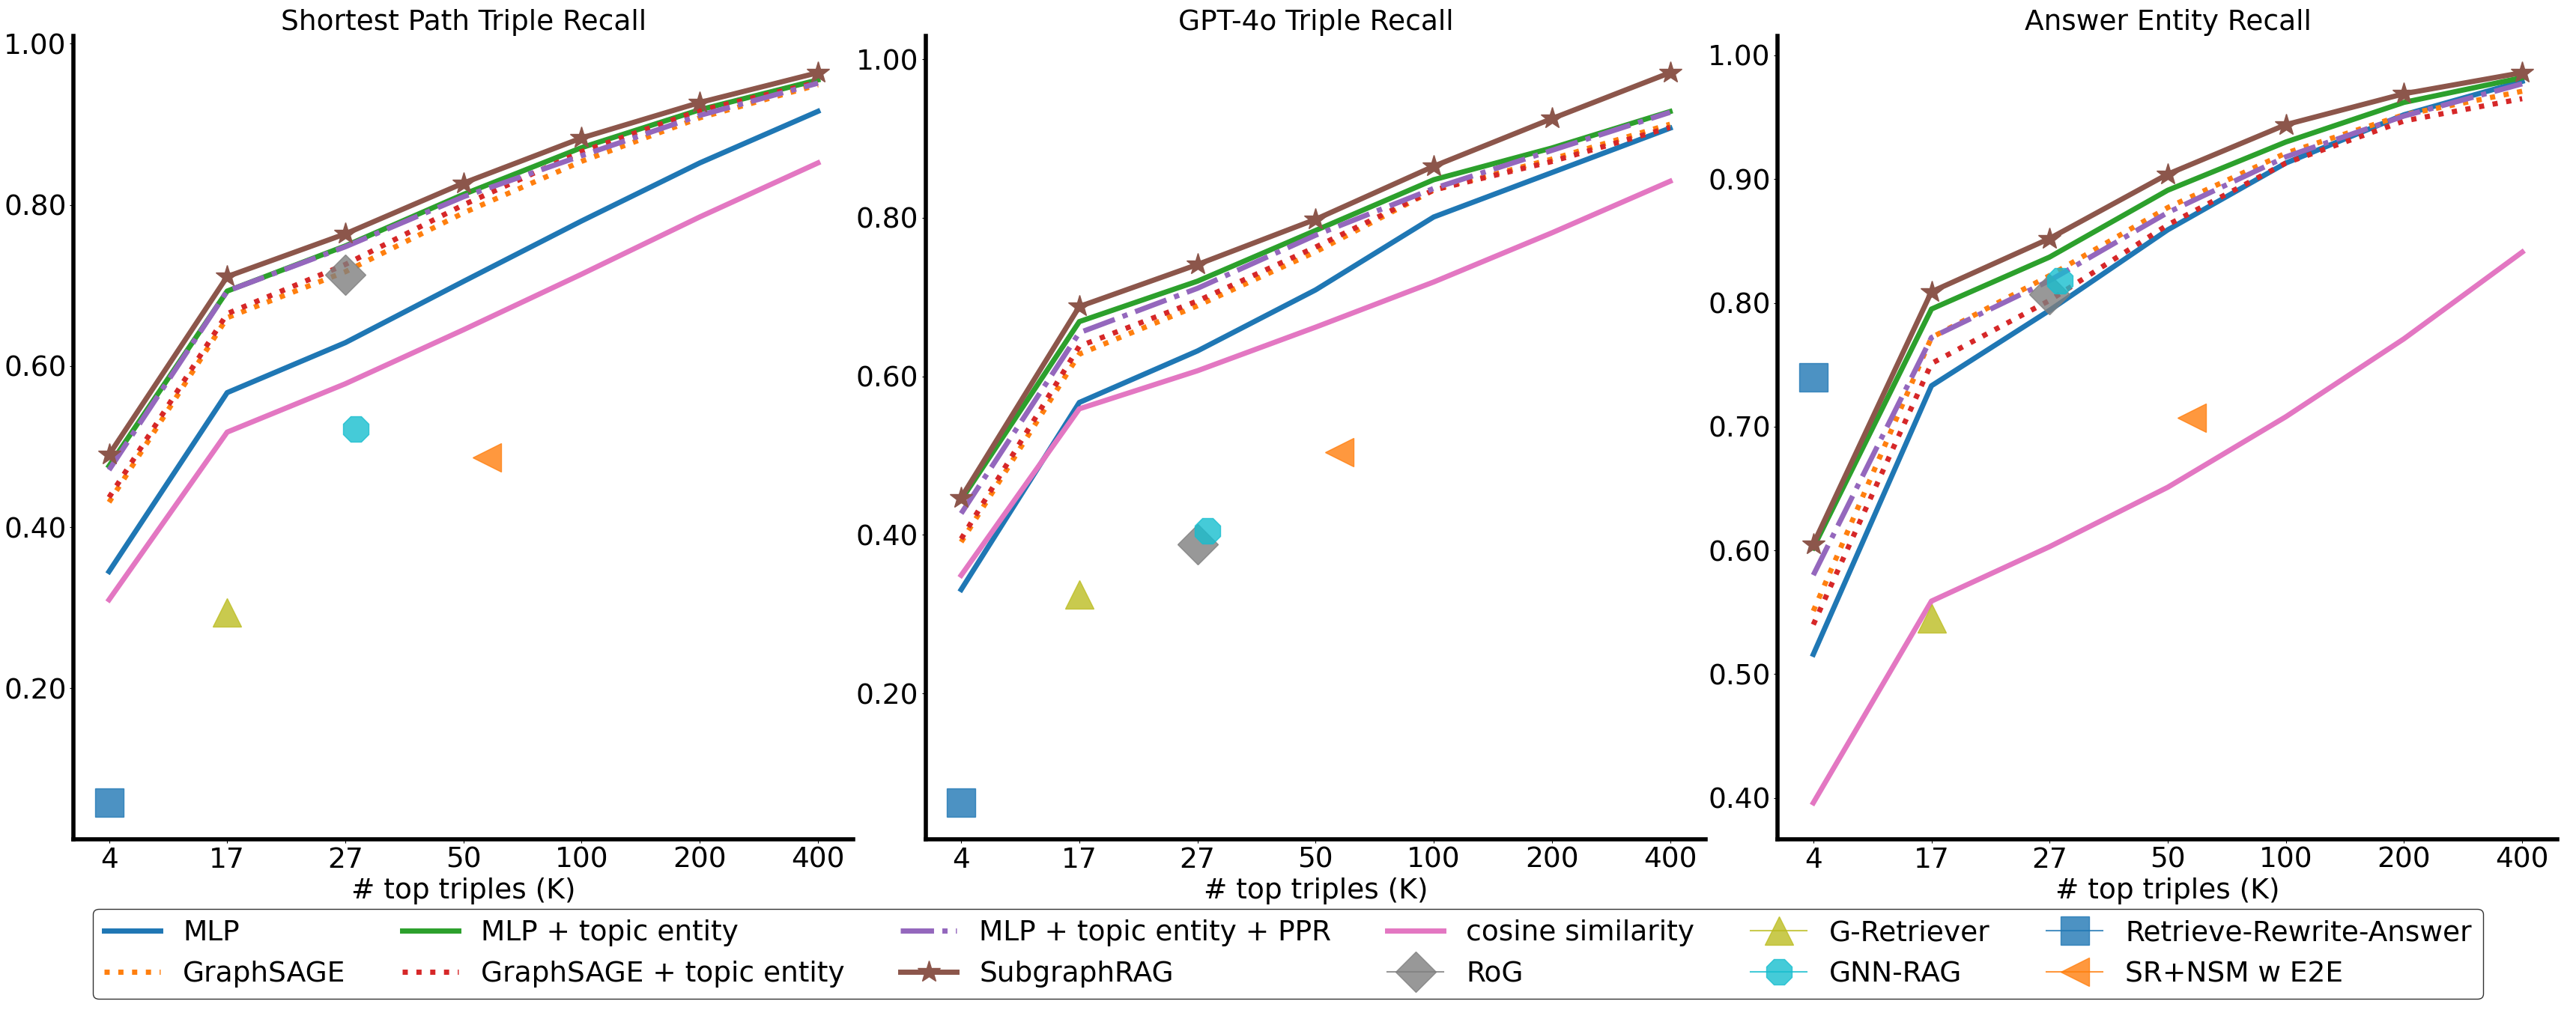
\includegraphics[trim={0.0cm 0cm 0.0cm 0cm}, clip, width=0.85\textwidth]{figs/webqsp_recall_k_SR.png}
    \vspace{-3mm}
    \caption{Retrieval effectiveness on WebQSP across various $K$ values for top-$K$ triple retrieval.}
    \label{fig:webqsp_k_recall}
\end{figure*}

Fig.~\ref{fig:webqsp_k_recall} presents the performance of \proj variants on WebQSP across a spectrum of $K$ values for top-$K$ triple retrieval, which is consistent with the observations made for CWQ.

\subsection{Evaluation Breakdown Over Topic Entity Count}
\label{appendix:break_topic}

\begin{table}[t]
\caption{Breakdown of recall evaluation for CWQ over topic entity count. Best results are in \underline{\textbf{bold}}.}
\vspace{-4mm}
\centering
\begin{adjustbox}{width=0.6\textwidth}
\begin{tabular}{lcccccc}
\\
\toprule
Model & \multicolumn{2}{c}{Shortest Path Triples} & \multicolumn{2}{c}{GPT-4o-labeled Triples} & \multicolumn{2}{c}{Answer Entities}\\
        \cmidrule(lr){2-3} \cmidrule(lr){4-5}
        \cmidrule(lr){6-7}
      & Single 
      & Multiple 
      & Single
      & Multiple 
      & Single
      & Multiple \\
      & $(46.3 \%)$
      & $(53.7 \%)$
      & $(46.3 \%)$
      & $(53.7 \%)$
      & $(46.3 \%)$
      & $(53.7 \%)$ \\
\midrule
cosine similarity
& $0.586$
& $0.403$
& $0.587$
& $0.499$
& $0.517$
& $0.638$\\
RoG 
& $0.711$
& $0.547$ 
& $0.324$
& $0.275$
& $0.769$
& $0.903$ \\
G-Retriever 
& $0.245$
& $0.128$
& $0.289$
& $0.156$
& $0.393$
& $0.360$ \\
% ReaRev + SBERT 
% & $0.475$
% & $0.484$
% & $0.354$
% & $0.381$
% & $0.786$
% & $0.819$ \\
% ReaRev + LMSR 
% & $0.472$
% & $0.486$
% & $0.355$
% & $0.387$
% & $0.792$
% & $0.827$\\
GNN-RAG 
& $0.496$
& $0.503$
& $0.369$
& $0.403$
& $0.829$
& $0.851$\\
\midrule
MLP 
& $0.788$
& $0.568$ 
& $0.777$
& $0.600$ 
& $0.894$
& $0.873$ \\
MLP + topic entity 
& $0.858$
& $0.690$ 
& $0.819$
& $0.718$
& $0.894$
& $0.889$ \\
\proj 
& $\underline{\mathbf{0.877}}$
& $\underline{\mathbf{0.754}}$
& 
$\underline{\mathbf{0.871}}$& $\underline{\mathbf{0.820}}$& $\underline{\mathbf{0.911}}$
& $\underline{\mathbf{0.916}}$ \\
\bottomrule
\end{tabular}
\end{adjustbox}
\label{tab: cwq_topic}
\end{table}

See table~\ref{tab: cwq_topic}.

\begin{figure*}[t]
    \vspace{-2mm}
    \centering
    \begin{subfigure}[t]{0.48\linewidth} 
        \centering
        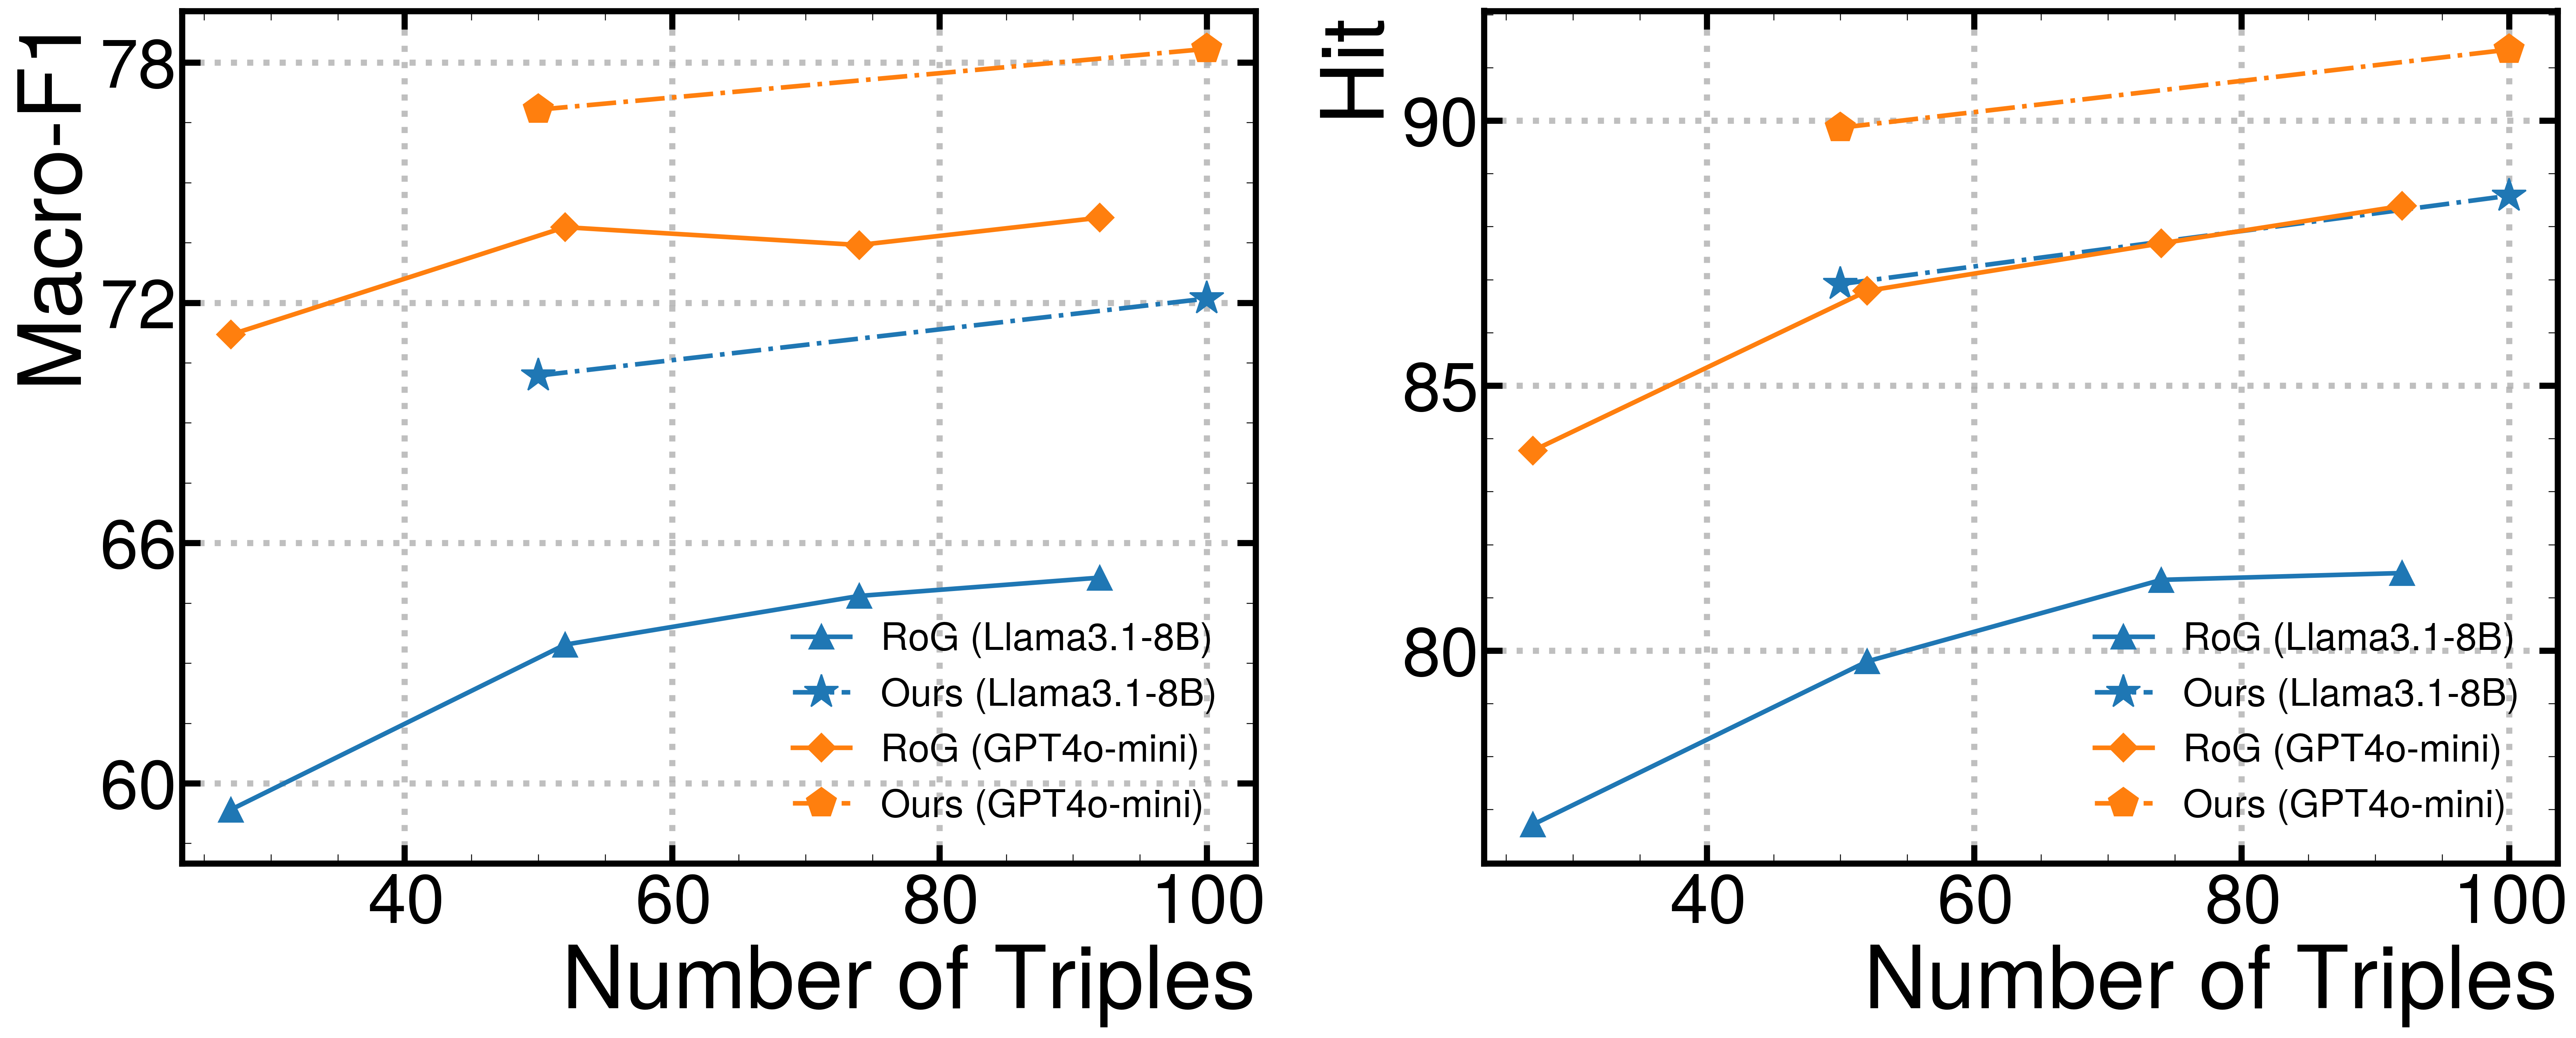
\includegraphics[trim={0cm 0.0cm 0cm 0.0cm}, clip, width=1.0\textwidth]{figs/numbers_webqsp_rog.png}
        \caption{WebQSP-sub}
    \end{subfigure}
    \hspace{0.01\linewidth}
    \begin{subfigure}[t]{0.48\linewidth}
        \centering
        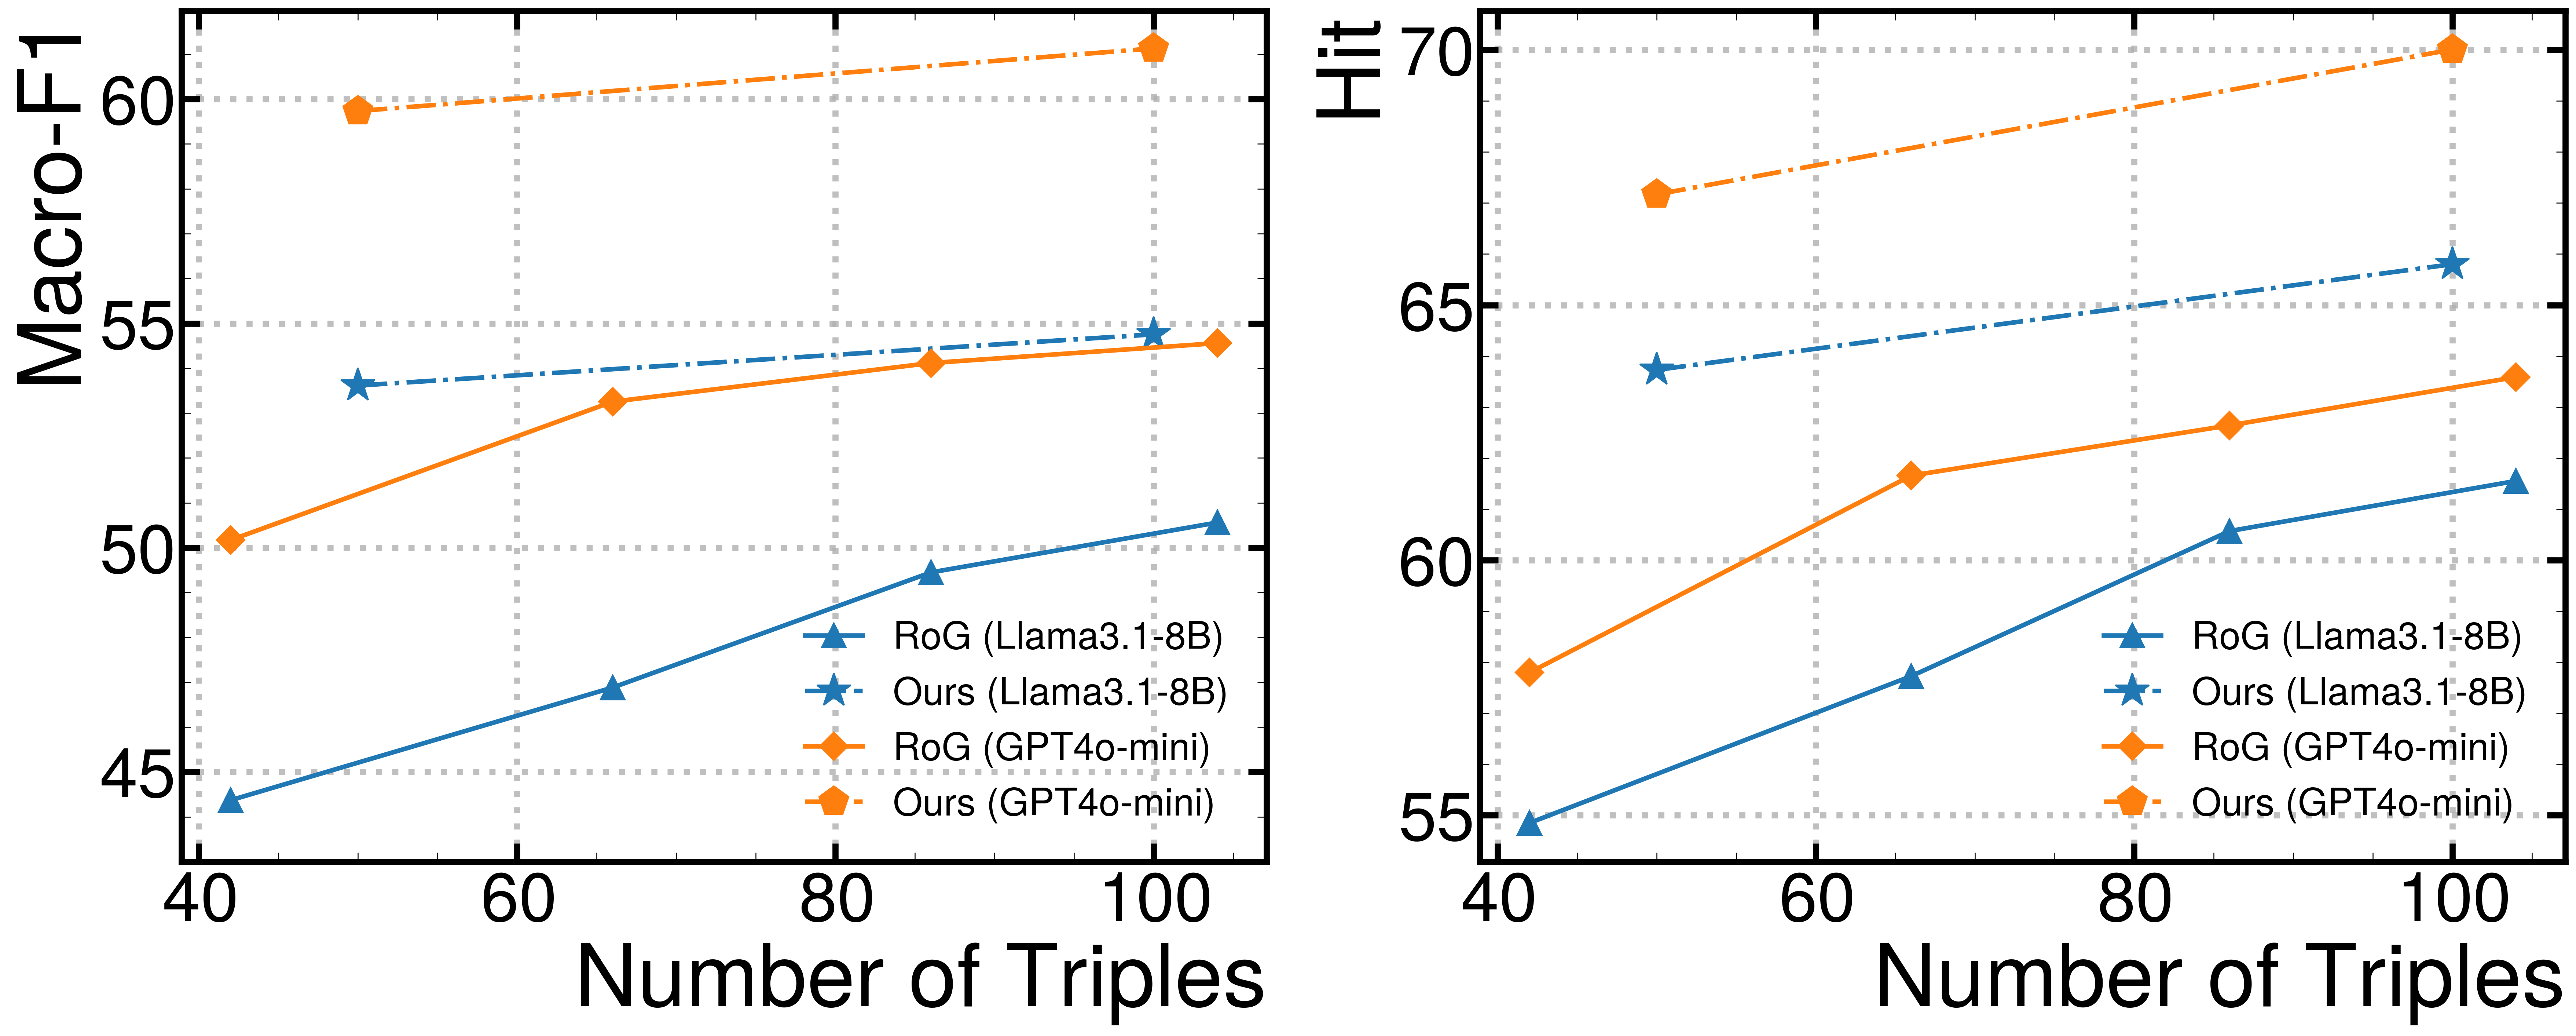
\includegraphics[trim={0cm 0.0cm 0.0cm 0cm}, clip,width=1.0\linewidth]{figs/numbers_cwq_rog.png}
        % \vspace*{-6mm}
        \caption{CWQ-sub}
    \end{subfigure}
    \vspace*{-2mm}
    \caption{Ablation studies on the number of retrieved triples and the used retrievers in SubgraphRAG. The triples from RoG's retriever are generated using beam search with sizes \{3, 6, 9, 12\}, and all the experiments use SubgraphRAG's un-fine-tuned LLM reasoners.}
    \label{fig:ablation_number_rog}
\end{figure*}

\section{Supplementary KGQA Results}\label{appx:score}

\textbf{Truth-grounded QA Analysis.} Table~\ref{tab:qa_breakdown} provides a detailed analysis of truth-grounding in generated answers, showing that previous methods often produce correct answers that are unsupported by the retrieved results, increasing the risk of hallucination. In particular, our method is significantly less likely to generate answers that are not present in the retriever results (the NR answers in the table). For instance, on CWQ-sub, more than 10\% of RoG’s correct answers are NR, while \proj keeps this to just 1\%. \proj can also decline to answer when there is insufficient evidence, with refusal rates increasing from 2\% to 19\% on WebQSP and from 7\% to 29\% on CWQ for questions lacking answers in the KG, compared to questions with KG-supported answers.  In contrast, baseline models consistently provide answers even when supporting evidence is absent. Together, these qualities make \proj a more trustworthy and truth-grounded KGQA framework.

To obtain a single metric to assess the degree of truth-grounded QA performance, we follow~\citep{yang2024crag} to develop a scoring strategy to aggregate the results of these tables. Specifically, for samples with answer entities present in the KG, correct answers receive a score of +1, incorrect answers -1, and missing answers 0. For samples without answer entities in the KG, missing answers, answers with entities found in the retrieved results, and answers with entities not found in the retrieved results are scored +1, -1, and -1.5, respectively. Denote $s_i$ as the score yielded for sample $i$ and $a_i$ the number of answers outputted by the LLM reasoner for this sample. For a dataset with $n$ samples:
$\text{Score}_{h} = \operatorname{Normalize} \left( \frac{1}{n} \sum_{i=0}^{n} \frac{s_i}{a_i} \right)$, where we use min-max normalization with $\text{min} = 0$ and $\text{max} = 100$. 
This metric penalizes hallucinated answers while favoring missing answers over incorrect ones.

\textbf{Impact of Retrieval Size.} Fig.~\ref{fig:ablation_number} shows how our SubgraphRAG would perform with different numbers of retrieved triples. To further demonstrate the superior performance of our proposed retriever module, we also scale RoG's retriever with more retrieved triples by increasing its beam search sizes (noting that this substantially increases computational costs). As shown in Fig.~\ref{fig:ablation_number_rog}, clearly, even when using RoG's retriever with more triples in SubgraphRAG, our proposed retriever consistently achieves significantly better results, further demonstrating the effectiveness of our retriever module. 

\begin{table}[t]
\caption{
Detailed performance of truth-grounded QA. No Ans Samples refers to cases where LLM reasoners refuse to answer; NR (Not Retrieved) indicates answers not present in the retrieved triples, while R (Retrieved) indicates answers found within the retrieved triples.}
\vspace{-3mm}
\label{tab:qa_breakdown}
\centering
\begin{adjustbox}{width=\textwidth}
\begin{tabular}{llcccccccc}
\\
\toprule
\multirow{2}{*}{Dataset} & \multirow{2}{*}{Method} & \multicolumn{4}{c}{Samples w/ Ans Entities in KG} & \multicolumn{3}{c}{Samples w/o Ans Entities in KG} \\
\cmidrule(lr){3-6} \cmidrule(lr){7-9}
&  & $\frac{\text{No Ans Samples}}{\text{Total Samples}}$  & $\frac{\text{Wrong Ans}}{\text{Total Ans}}$  & $\frac{\text{Correct Ans (NR) }}{\text{Correct Ans}}$ & $\frac{\text{Wrong Ans (NR)}}{\text{Wrong Ans}}$ & $\frac{\text{No Ans Samples }}{\text{Total Samples}}$ & $\frac{\text{Wrong Ans (NR)}}{\text{Total Ans}}$ & $\frac{\text{Wrong Ans (R)}}{\text{Total Ans}}$\\
\midrule
\multirow{4}{*}{\shortstack{WebQSP}} 
& RoG-Joint & 0/1559 = 0\% & 4605/10206 = 45\% & 170/5601 = 3\% & 1178/4605 = 26\% & 0/69 = 0\% & 24/126 = 19\% & 70/126 = 56\% \\
& RoG-Sep & 0/1559 = 0\% & 6867/12401 = 55\% & 327/5534 = 6\% & 2494/6867 = 36\% & 0/69 = 0\% & 71/162 = 44\% & 43/162 = 27\% \\
\cmidrule(lr){2-9}
& \proj (Llama3.1-8B) & 29/1559 = 2\% & 1397/5850 = 24\% & 59/4453 = 1\% & 84/1397 = 6\% & 13/69 = 19\% & 16/107 = 15\% & 71/107 = 66\% \\
& \proj (GPT4o-mini) & 12/1559 = 1\% & 1802/8011 = 22\% & 37/6209 = 1\% & 126/1802 = 7\% & 7/69 = 10\% & 17/83 = 20\% & 31/83 = 37\% \\
\toprule
\multirow{4}{*}{\shortstack{CWQ}} 
& RoG-Joint & 0/2848 = 0\% & 3651/6709 = 54\% & 305/3058 = 10\% & 1293/3651 = 35\% & 0/683 = 0\% & 1835/2729 = 67\% & 363/2729 = 13\% \\
& RoG-Sep & 0/2848 = 0\% & 3183/6129 = 52\% & 341/2946 = 12\% & 1295/3183 = 41\% & 0/683 = 0\% & 1840/2620 = 70\% & 268/2620 = 10\% \\
\cmidrule(lr){2-9}
& \proj (Llama3.1-8B) & 210/2848 = 7\% & 2417/5028 = 48\% & 21/2611 = 1\% & 98/2417 = 4\% & 199/683 = 29\% &  114/1052 = 11\% & 819/1052 = 78\% \\
& \proj (GPT4o-mini) & 203/2848 = 7\% & 2194/5205 = 42\% & 30/3011 = 1\% & 159/2194 = 7\% & 137/683 = 20\%  & 170/953 = 18\% & 564/953 = 59\% \\
\bottomrule
\end{tabular}
\end{adjustbox}
\vspace{-4mm}
\end{table}

\begin{table}[t]
\caption{Ablation studies with different retrievers, using the same prompt and GPT4o-mini as the reasoner. Rand refers to random triple sampling, RandNoAns removes triples with ground-truth answers after random sampling, and NoRetriever directly asks questions without KG info.}
\vspace{-4mm}
\label{tab:ablation_retriever_4omini}
\centering
\begin{adjustbox}{width=\textwidth}
\begin{tabular}{rcccccccccccccc}
\\
\toprule
 & \multicolumn{2}{c}{WebQSP} & \multicolumn{2}{c}{CWQ} & \multicolumn{5}{c}{WebQSP-sub} & \multicolumn{5}{c}{CWQ-sub} \\
\cmidrule(lr){2-3} \cmidrule(lr){4-5}  \cmidrule(lr){6-10} \cmidrule(lr){11-15}
      & Macro-F1     & Hit & Macro-F1 & Hit & Macro-F1 & Micro-F1 & Hit & Hit@1 & Score$_{h}$ & Macro-F1 & Micro-F1 & Hit & Hit@1 & Score$_{h}$\\
\midrule
Rand + \proj Reasoner
& 47.70 & 68.37 & 33.13 & 39.82 & 47.15 & 23.74 & 68.57 & 64.59 & 69.67 & 35.55 & 34.26 & 42.94 & 40.48 & 54.81
\\

 

RandNoAns + \proj Reasoner
& 36.83 & 49.63 & 25.69 & 30.70 & 35.77 & 14.62 & 48.94 & 44.96 & 57.12 & 26.25 & 26.11 & 31.60 & 29.21 & 48.80
\\


NoRetriever + \proj Reasoner
& 47.49 & 71.01 & 33.43 & 42.25 & 46.68 & 25.53 & 70.94 & 62.67 & 60.22 & 35.66 & 31.11 & 44.66 & 39.99 & 44.24
\\



\midrule

cosine similarity + \proj Reasoner
& 64.94 & 78.19 & 41.23 & 49.22 & 65.26 & 43.84 & 78.90 & 74.15 & 73.03 & 45.07 & 42.27 & 53.83 & 49.37 & 57.06
\\ 


Retrieve-Rewrite-Answer + \proj Reasoner 
& 38.26 & 53.62 & - & - & 37.54 & 19.62 & 53.37 & 50.10 & 67.68 & - & - & - & - & -
\\ 

StructGPT + \proj Reasoner
& 71.62 & 82.68 & - & - & 71.66 & 59.05 & 82.87 & 80.44 & 81.48 & - & - & - & - & -
\\

G-Retriever + \proj Reasoner
& 59.28 & 75.25 & 36.79 & 42.23 & 59.55 & 35.19 & 76.01 & 72.87 & 76.31 & 39.55 & 39.42 & 45.47 & 43.29 & 57.67
\\ 


RoG-Sep + \proj Reasoner  
& 70.08 & 82.25 & 44.30 & 51.15 & 70.91 & 54.69 & 83.45 & 78.51 & 81.00 & 49.85 & 50.40 & 57.51 & 52.35 & 64.27
\\

GNN-RAG + \proj Reasoner 
& 73.27 & 85.93 & 52.91 & 59.64 & 74.24 & 53.92 & 87.24 & 83.39 & 84.41 & 60.89 & 59.86 & 68.43 & 64.04 & 67.71
\\

GNN-RAG ($\leftrightarrow$) + \proj Reasoner 
& 61.19 & 78.99 & 43.42 & 51.37 & 61.41 & 42.02 & 79.79 & 74.98 & 76.11 & 48.04 & 43.7 & 56.88 & 52.32 & 59.45
\\


\midrule
\proj
& 77.45 & 90.11 & 54.13 & 62.02 & 78.34 & 58.44 & 91.34 & 87.36 & 82.21 & 61.13 & 58.86 & 70.01 & 65.48 & 64.20
\\

\proj ($\leftrightarrow$) & 73.81 & 88.08 & 44.69 & 54.21 & 74.42 & 49.41 & 89.10 & 84.67 & 81.35 & 49.47 & 45.16 & 60.18 & 54.18 & 58.86
\\

\bottomrule
\end{tabular}
\end{adjustbox}
\vspace{0mm}
\end{table}

\section{Prompt Templates}\label{appendix:prompt}
Fig.~\ref{fig:prompt_qa_detailed} is the detailed prompt template used in our experiments for all samples, and Fig.~\ref{fig:prompt_gpt4_label} provides the prompt employed to label relevant triples via GPT-4o.

\begin{wrapfigure}{l}{1\textwidth}
\begin{tcolorbox}[colback=gray!5!white, colframe=gray!75!black, title=Input Prompts for KGQA]
\scriptsize

\textbf{System:}\\
\raggedright Based on the triples retrieved from a knowledge graph, please answer the question. Please return formatted answers as a list, each prefixed with ``ans:".
% \vspace{-1mm}
\rule{\linewidth}{0.4pt} 
\\
\textbf{User:} \; {\color{red}{// ICL example}} \\
Triplets:

(Lou Seal,sports.mascot.team,San Francisco Giants)

(San Francisco Giants,sports.sports\_team.championships,2012 World Series)

(San Francisco Giants,sports.sports\_championship\_event.champion,2014 World Series)

(San Francisco Giants,time.participant.event,2014 Major League Baseball season)

(San Francisco Giants,time.participant.event,2010 World Series)

(San Francisco Giants,time.participant.event,2010 Major League Baseball season)

(San Francisco Giants,sports.sports\_team.championships,2014 World Series)

(San Francisco Giants,sports.sports\_team.team\_mascot,Crazy Crab)

(San Francisco Giants,sports.sports\_team.championships,2010 World Series)

(San Francisco Giants,sports.professional\_sports\_team.owner\_s,Bill Neukom)

(San Francisco Giants,time.participant.event,2012 World Series)

(San Francisco,sports.sports\_team\_location.teams,San Francisco Giants)

(San Francisco Giants,sports.sports\_team.arena\_stadium,AT\&T Park)

(AT\&T Park,location.location.events,2012 World Series)

...
\vspace{1mm}
\\

Question:

What year did the team with mascot named Lou Seal win the World Series?
\\
\rule{\linewidth}{0.4pt} 
\\
\textbf{Assistant:} \; {\color{red}{// ICL example}} 

To find the year the team with mascot named Lou Seal won the World Series, we need to find the team with mascot named Lou Seal and then find the year they won the World Series.\\

From the triplets, we can see that Lou Seal is the mascot of the San Francisco Giants.\\

Now, we need to find the year the San Francisco Giants won the World Series.\\

From the triplets, we can see that San Francisco Giants won the 2010 World Series and 2012 World Series and 2014 World Series.\\

So, the team with mascot named Lou Seal (San Francisco Giants) won the World Series in 2010, 2012, and 2014.\\

Therefore, the formatted answers are:\\

ans: 2014 (2014 World Series)\\
ans: 2012 (2012 World Series)\\
ans: 2010 (2010 World Series)\\
\rule{\linewidth}{0.4pt} 
\textbf{User:}\; {\color{red}{// Sample to infer}} 

Triplets:\\
(e$_{a}$, r$_{ab}$, e$_b$) \; {\color{red}{// Retrieved triples}} \\
(e$_{c}$, r$_{cd}$, e$_d$)\\
\dots\\
Question:\\
what's \dots? \;  {\color{red}{// Q in datasets}}
\end{tcolorbox}
\vspace{-3mm}
\caption{Detailed prompt for LLM question-answering used in our experiments for all samples.}
\label{fig:prompt_qa_detailed}
\end{wrapfigure}

\begin{wrapfigure}{l}{1.0\textwidth}
\begin{tcolorbox}[colback=gray!5!white, colframe=gray!75!black, title=Input Prompts for Labeling Relevant Triples via GPT-4o]
\scriptsize

\textbf{System:}\\
\raggedright Based on the triplets retrieved from a knowledge graph, please select relevant triplets for answering the question. Please return formatted triplets as a list, each prefixed with "evidence:".
% \vspace{-1mm}
\rule{\linewidth}{0.4pt} 
\\
\textbf{User:}\; {\color{red}{// Sample to infer}} 

Triplets:\\
(e$_{a}$, r$_{ab}$, e$_b$) \; {\color{red}{// Retrieved triples}} \\
(e$_{c}$, r$_{cd}$, e$_d$)\\
\dots\\
Question:\\
what's \dots? \;  {\color{red}{// Q in datasets}}
\end{tcolorbox}
\caption{Detailed prompt for labeling triples via GPT-4o.}
\label{fig:prompt_gpt4_label}
\end{wrapfigure}

\clearpage
\section{Explainablity Examples}\label{appx:explain}

To demonstrate the superior explainability of our approach, we provide multiple example responses from our LLM reasoners below, which cover questions requiring different reasoning hops and logic chains.
We have also included examples of our LLM reasoners refusing to answer due to insufficient information in Appendix~\ref{appx:refusal}, which helps to provide more truth-grounded answers. 
Due to limited space, we do not include retrieved triples for all the examples, but one will be able to find full prediction files in our released repository.

\subsection{LLM Responses with Explainable Reasoning}

% a->b->c
\begin{wrapfigure}{l}{1.0\textwidth}
\begin{tcolorbox}[colback=gray!5!white, colframe=gray!75!black, title=CWQ-WebQTest-100\_bf66fd89b6e9fc5fcb96c8b3f7a0e616]
\scriptsize

\textbf{Question:}\\
\raggedright The people from the country that contains Nord-Ouest Department speak what languages today?

\rule{\linewidth}{0.4pt}
\\

\textbf{Retrieved Triples:}\\
(Haiti,location.country.languages\_spoken,Haitian Creole)

(Haiti,location.country.first\_level\_divisions,Nord-Ouest Department)

(Haiti,location.country.official\_language,French)

(French,language.human\_language.countries\_spoken\_in,Haiti)

(Nord-Ouest Department,location.administrative\_division.first\_level\_division\_of,Haiti)

(Haiti,location.country.languages\_spoken,French)

(Haiti,location.country.administrative\_divisions,Nord-Ouest Department)

(Haiti,location.country.official\_language,Haitian Creole)

(Nord-Ouest Department,location.location.containedby,Haiti)

(Haitian Creole,language.human\_language.main\_country,Haiti)

...

\rule{\linewidth}{0.4pt}
\\

\textbf{LLM Response:}\\
To find the languages spoken in the country that contains Nord-Ouest Department, we need to find the country that contains Nord-Ouest Department.



From the triplets, we can see that Nord-Ouest Department is contained by Haiti.



So, the country that contains Nord-Ouest Department is Haiti.



From the triplets, we can see that Haiti speaks Haitian Creole and French.



Therefore, the people from the country that contains Nord-Ouest Department (Haiti) speak Haitian Creole and French today.



The formatted answer is:



ans: Haitian Creole

ans: French

\rule{\linewidth}{0.4pt}
\\
\textbf{Ground-truth:}\\
Haitian Creole

French

\end{tcolorbox}
\end{wrapfigure}



% a->b->c
\begin{wrapfigure}{l}{1.0\textwidth}
\begin{tcolorbox}[colback=gray!5!white, colframe=gray!75!black, title=CWQ-WebQTest-1320\_c5498ca807d2e1ec30d4c8fdd41f0bf7]
\scriptsize

\textbf{Question:}\\
\raggedright What stadium does the team with mascot named Hank play at?

\rule{\linewidth}{0.4pt}
\\

\textbf{Retrieved Triples:}\\
(Milwaukee Brewers,sports.sports\_team.team\_mascot,Hank)

(Hank,sports.mascot.team,Milwaukee Brewers)

(Milwaukee Brewers,sports.sports\_team.previously\_known\_as,Seattle Pilots)

(Seattle Pilots,sports.defunct\_sports\_team.later\_known\_as,Milwaukee Brewers)

(Milwaukee Brewers,sports.sports\_team.arena\_stadium,Miller Park)

(Milwaukee Brewers,sports.sports\_team.location,Milwaukee)

(Miller Park,sports.sports\_facility.teams,Milwaukee Brewers)

(Milwaukee,sports.sports\_team\_location.teams,Milwaukee Brewers)

(Miller Park,location.location.containedby,Milwaukee)

(Milwaukee Brewers,baseball.baseball\_team.current\_coaches,m.0527c88)

...

\rule{\linewidth}{0.4pt}
\\

\textbf{LLM Response:}\\
To find the stadium where the team with mascot named Hank plays, we need to find the team with mascot named Hank and then find the stadium they play at.



From the triplets, we can see that Hank is the mascot of the Milwaukee Brewers.



Now, we need to find the stadium where the Milwaukee Brewers play.



From the triplets, we can see that the Milwaukee Brewers play at Miller Park.



Therefore, the formatted answer is:



ans: Miller Park

\rule{\linewidth}{0.4pt}
\\
\textbf{Ground-truth:}\\
Miller Park

\end{tcolorbox}
\end{wrapfigure}





% a->b->c
\begin{wrapfigure}{l}{1.0\textwidth}
\begin{tcolorbox}[colback=gray!5!white, colframe=gray!75!black, title=CWQ-WebQTrn-2152\_92fba37c9723caee68665ad9a5e4a468]
\scriptsize

\textbf{Question:}\\
\raggedright Which of team owners Tom Hicks sports team are in the American League West?

\rule{\linewidth}{0.4pt}
\\

\textbf{Retrieved Triples:}\\
(Texas Rangers,sports.professional\_sports\_team.owner\_s,Tom Hicks)

(Tom Hicks,sports.sports\_team\_owner.teams\_owned,Texas Rangers)

(Dallas Stars,sports.professional\_sports\_team.owner\_s,Tom Hicks)

(Seattle Pilots,sports.defunct\_sports\_team.later\_known\_as,Milwaukee Brewers)

(Tom Hicks,sports.sports\_team\_owner.teams\_owned,Dallas Stars)

(United States of America,base.locations.countries.states\_provinces\_within,Alabama)

(Houston Astros,sports.professional\_sports\_team.owner\_s,Drayton McLane, Jr.)

(m.0crtd2r,sports.sports\_league\_participation.team,Los Angeles Angels of Anaheim)

(United States of America,base.aareas.schema.administrative\_area.administrative\_children,Alabama)

(m.0crtd31,sports.sports\_league\_participation.team,Anaheim Angels)

(United States of America,base.aareas.schema.administrative\_area.administrative\_children,Washington, D.C.)

(United States of America,base.locations.countries.states\_provinces\_within,Mississippi)

(m.0crtd3v,sports.sports\_league\_participation.team,California Angels)

(United States of America,base.aareas.schema.administrative\_area.administrative\_children,Mississippi)

(American League West,baseball.baseball\_division.teams,Texas Rangers)

...

\rule{\linewidth}{0.4pt}
\\

\textbf{LLM Response:}\\
To find the teams owned by Tom Hicks that are in the American League West, we need to find the teams owned by Tom Hicks and then find the teams in the American League West.



From the triplets, we can see that Tom Hicks owns the Texas Rangers and Dallas Stars.



Now, we need to find the teams in the American League West.



From the triplets, we can see that the teams in the American League West are Texas Rangers, Los Angeles Angels of Anaheim, Seattle Mariners, Oakland Athletics, and Seattle Pilots.



So, among the teams owned by Tom Hicks (Texas Rangers and Dallas Stars), only Texas Rangers is in the American League West.



Therefore, the formatted answer is:



ans: Texas Rangers

\rule{\linewidth}{0.4pt}
\\
\textbf{Ground-truth:}\\
Texas Rangers

\end{tcolorbox}
\end{wrapfigure}




% a->b->c->d
\begin{wrapfigure}{l}{1.0\textwidth}
\begin{tcolorbox}[colback=gray!5!white, colframe=gray!75!black, title=CWQ-WebQTrn-557\_960c16ffdb29e173df0577fc76c7455d]
\scriptsize

\textbf{Question:}\\
\raggedright In the film with the character named Winged Monkey \#7, who played Dorothy?

\rule{\linewidth}{0.4pt}
\\
\textbf{LLM Response:}\\
To find the actor who played Dorothy in the film with the character named Winged Monkey \#7, we need to find the film that Winged Monkey \#7 is in and then find the actor who played Dorothy in that film.



From the triplets, we can see that Winged Monkey \#7 is in the film "The Wizard of Oz" (m.0yj6tr7).



Now, we need to find the actor who played Dorothy in "The Wizard of Oz".



From the triplets, we can see that Judy Garland (m.0k6y72) played Dorothy in "The Wizard of Oz".



Therefore, the formatted answer is:



ans: Judy Garland

\rule{\linewidth}{0.4pt}
\\
\textbf{Ground-truth:}\\
Judy Garland

\end{tcolorbox}
 

\end{wrapfigure}


% a->c & b->c
\begin{wrapfigure}{l}{1.0\textwidth}
\begin{tcolorbox}[colback=gray!5!white, colframe=gray!75!black, title=CWQ-WebQTrn-2904\_cb8d941f825c5dd7b2d6f3faef7f9229]
\scriptsize

\textbf{Question:}\\
\raggedright What city is home for Lauren Conrad and had a mayor named Willie Brown?

\rule{\linewidth}{0.4pt}
\\
\textbf{LLM Response:}\\
To find the city that is home for Lauren Conrad and had a mayor named Willie Brown, we need to find the city where Lauren Conrad lives and the city where Willie Brown was the mayor.



From the triplets, we can see that Lauren Conrad lived in Los Angeles (m.043jjv4) and San Francisco (m.04hy\_14).



From the triplets, we can see that Willie Brown was the mayor of San Francisco.



Therefore, the city that is home for Lauren Conrad and had a mayor named Willie Brown is San Francisco.



So, the formatted answer is:



ans: San Francisco

\rule{\linewidth}{0.4pt}
\\
\textbf{Ground-truth:}\\
San Francisco

\end{tcolorbox}
 

\end{wrapfigure}







\begin{wrapfigure}{l}{1.0\textwidth}
\begin{tcolorbox}[colback=gray!5!white, colframe=gray!75!black, title=CWQ-WebQTrn-124\_405a78f132e69f4771aff40d07cd0294]
\scriptsize

\textbf{Question:}\\
\raggedright Which movie did Angelina Jolie direct, that was produced by Erwin Stoff?

\rule{\linewidth}{0.4pt}
\\
\textbf{LLM Response:}\\
To find the movie that Angelina Jolie directed, which was produced by Erwin Stoff, we need to find the movies that Angelina Jolie directed and the movies that Erwin Stoff produced.



From the triplets, we can see that Angelina Jolie directed the following movies:

- In the Land of Blood and Honey

- Unbroken

- By the Sea



From the triplets, we can see that Erwin Stoff produced the following movies:

- Unbroken

- The Day the Earth Stood Still

- Edge of Tomorrow

- Water for Elephants

- Austin Powers: The Spy Who Shagged Me

- The Blind Side

- The Replacements

- I Am Legend

- Hardball

- The Lake House

- Street Kings

- 47 Ronin



Now, we need to find the common movie between Angelina Jolie's directed movies and Erwin Stoff's produced movies.



The common movie is Unbroken.



Therefore, the formatted answer is:



ans: Unbroken

\rule{\linewidth}{0.4pt}
\\
\textbf{Ground-truth:}\\
Unbroken

\end{tcolorbox}
 

\end{wrapfigure}



% a->b
\begin{wrapfigure}{l}{1.0\textwidth}
\begin{tcolorbox}[colback=gray!5!white, colframe=gray!75!black, title=WebQSP-WebQTest-33]
\scriptsize

\textbf{Question:}\\
\raggedright what timezone is sweden

\rule{\linewidth}{0.4pt}
\\

\textbf{Retrieved Triples:}\\
(Sweden,location.location.time\_zones,Central European Time Zone)

(Sweden,location.country.languages\_spoken,Finnish Language)

(Finnish Language,language.human\_language.countries\_spoken\_in,Sweden)

(Sweden,location.country.languages\_spoken,Turoyo Language)

(Sweden,location.country.official\_language,Swedish Language)

(Spain,location.location.time\_zones,Central European Time Zone)

(Stockholm,location.location.time\_zones,Central European Time Zone)

(Unitary state,government.form\_of\_government.countries,Sweden)

(Swedish Language,language.human\_language.countries\_spoken\_in,Finland)

(Sweden,location.country.languages\_spoken,Swedish Language)

...

\rule{\linewidth}{0.4pt}
\\

\textbf{LLM Response:}\\
To find the timezone of Sweden, we can look for the triplets that contain Sweden and have a property related to timezones.



From the triplets, we can see that Sweden is located in the Central European Time Zone.



Therefore, the answer is:



ans: Central European Time Zone

\rule{\linewidth}{0.4pt}
\\
\textbf{Ground-truth:}\\
Central European Time Zone

\end{tcolorbox}
\end{wrapfigure}







\begin{wrapfigure}{l}{1.0\textwidth}
\begin{tcolorbox}[colback=gray!5!white, colframe=gray!75!black, title=WebQSP-WebQTest-188]
\scriptsize

\textbf{Question:}\\
\raggedright where did bristol palin go to school

\rule{\linewidth}{0.4pt}
\\

\textbf{Retrieved Triples:}\\
(m.0byl4zl,education.education.institution,Wasilla High School)

(Wasilla High School,education.educational\_institution.students\_graduates,m.0byl4zl)

(Juneau-Douglas High School,education.educational\_institution.students\_graduates,m.0cpkbwp)

(m.0cpkbwp,education.education.institution,Juneau-Douglas High School)

(Bristol Palin,people.person.education,m.0byl4zl)

(Bristol Palin,people.person.education,m.0cpk4bl)

(Bristol Palin,people.person.education,m.0cpkbwp)

(m.0cpk4bl,education.education.institution,West Anchorage High School)

(West Anchorage High School,education.educational\_institution.students\_graduates,m.0cpk4bl)

(m.0byl4zl,education.education.student,Bristol Palin)

(m.0cpk4bl,education.education.student,Bristol Palin)

(m.0cpkbwp,education.education.student,Bristol Palin)

(m.04tlm1z,education.education.institution,Wasilla High School)

(m.0n1g77g,education.education.institution,Wasilla High School)

(Wasilla High School,education.educational\_institution.students\_graduates,m.04tlm1z)

(Wasilla High School,education.educational\_institution.students\_graduates,m.0n1g77g)

(Bristol Palin,people.person.place\_of\_birth,Wasilla)

(Wasilla,location.location.people\_born\_here,Bristol Palin)

(Bristol Palin,people.person.nationality,United States of America)

(Levi Johnston,people.person.place\_of\_birth,Wasilla)

...

\rule{\linewidth}{0.4pt}
\\

\textbf{LLM Response:}\\
To find where Bristol Palin went to school, we need to find the educational institutions that Bristol Palin attended.



From the triplets, we can see that Bristol Palin attended the following educational institutions:



- Wasilla High School (m.0byl4zl)

- Juneau-Douglas High School (m.0cpkbwp)

- West Anchorage High School (m.0cpk4bl)



Therefore, the formatted answers are:



ans: Wasilla High School

ans: Juneau-Douglas High School

ans: West Anchorage High School

\rule{\linewidth}{0.4pt}
\\
\textbf{Ground-truth:}\\
West Anchorage High School

Wasilla High School

Juneau-Douglas High School

\end{tcolorbox}
\end{wrapfigure}



\begin{wrapfigure}{l}{1.0\textwidth}
\begin{tcolorbox}[colback=gray!5!white, colframe=gray!75!black, title=WebQSP-WebQTest-760]
\scriptsize

\textbf{Question:}\\
\raggedright what party does barack obama belong to

\rule{\linewidth}{0.4pt}
\\

\textbf{Retrieved Triples:}\\
(Barack Obama,influence.influence\_node.influenced\_by,Saul Alinsky)

(Barack Obama,organization.organization\_founder.organizations\_founded,National Commission on Fiscal Responsibility and Reform)

(Barack Obama presidential campaign, 2012,government.election\_campaign.party,Democratic Party)

(Barack Obama,government.politician.election\_campaigns,Barack Obama presidential primary campaign, 2008)

(Barack Obama,government.politician.party,m.03gjhww)

(Barack Obama,government.politician.election\_campaigns,Barack Obama 1996 Illinois Senate Campaign)

(Barack Obama 2004 US Senate Campaign,government.election\_campaign.party,Democratic Party)

(Barack Obama,influence.influence\_node.influenced\_by,Reinhold Niebuhr)

(m.03gjhww,government.political\_party\_tenure.party,Democratic Party)

(Barack Obama,organization.organization\_founder.organizations\_founded,White House Task Force to Protect Students from Sexual Assault)

(Barack Obama presidential primary campaign, 2008,government.election\_campaign.party,Democratic Party)

(Barack Obama 1996 Illinois Senate Campaign,government.election\_campaign.party,Democratic Party)

(Barack Obama,base.politicalconventions.presidential\_nominee.nominated\_at,2008 Democratic National Convention)

(Barack Obama,government.politician.government\_positions\_held,m.03h96h6)

(Barack Obama,government.politician.election\_campaigns,Barack Obama 2004 US Senate Campaign)

...

\rule{\linewidth}{0.4pt}
\\

\textbf{LLM Response:}\\
From the triplets, we can see that Barack Obama is associated with the Democratic Party in several instances:



1. (Barack Obama,government.politician.party,m.03gjhww)

2. (Barack Obama 2004 US Senate Campaign,government.election\_campaign.party,Democratic Party)

3. (Barack Obama 1996 Illinois Senate Campaign,government.election\_campaign.party,Democratic Party)

4. (Barack Obama presidential primary campaign, 2008,government.election\_campaign.party,Democratic Party)

5. (Democratic Party presidential primaries, 2008,government.primary\_election.party,Democratic Party)

6. (m.03gjhww,government.political\_party\_tenure.party,Democratic Party)



Therefore, the formatted answer is:



ans: Democratic Party

\rule{\linewidth}{0.4pt}
\\
\textbf{Ground-truth:}\\
Democratic Party

\end{tcolorbox}
\end{wrapfigure}



\begin{wrapfigure}{l}{1.0\textwidth}
\begin{tcolorbox}[colback=gray!5!white, colframe=gray!75!black, title=WebQSP-WebQTest-62]
\scriptsize

\textbf{Question:}\\
\raggedright what was jesse james killed with

\rule{\linewidth}{0.4pt}
\\
\textbf{LLM Response:}\\
To find what Jesse James was killed with, we need to find the cause of his death.



From the triplets, we can see that Jesse James was killed by Assassination.



Now, we need to find the cause of Assassination.



From the triplets, we can see that Assassination includes causes of death such as Assassination in ways which appear natural, Assassination by 'Accident', Assassination by firearm, and Assassination by 'Suicide'.



However, we are looking for what Jesse James was killed with, not how he was killed. 



From the triplets, we can see that Firearm is a cause of death that includes causes of death such as Assassination by firearm.



Therefore, Jesse James was killed with a Firearm.



So, the answer is:



ans: Firearm

\rule{\linewidth}{0.4pt}
\\
\textbf{Ground-truth:}\\
Firearm

\end{tcolorbox}
\end{wrapfigure}


\clearpage
\subsection{LLM Refusal to Answer Due to Insufficient Information}
\label{appx:refusal}



\begin{wrapfigure}{l}{1.0\textwidth}
\begin{tcolorbox}[colback=gray!5!white, colframe=gray!75!black, title=WebQSP-WebQTest-386]
\scriptsize

\textbf{Question:}\\
\raggedright how deep is lake merritt oakland

\rule{\linewidth}{0.4pt}
\\
\textbf{LLM Response:}\\
To find the depth of Lake Merritt in Oakland, we need to look for any information related to the depth of Lake Merritt.



From the triplets, we can see that Lake Merritt is a lake, but there is no direct information about its depth.



However, we can see that Lake Merritt is a National Historic Landmark (m.06\_44f4, protected\_sites.natural\_or\_cultural\_site\_listing.designation\_as\_national\_or\_cultural\_site, m.06\_44f4) and a National Historic Landmark (m.06\_44f4, protected\_sites.natural\_or\_cultural\_site\_listing.category\_or\_criteria, National Historic Landmark).



We can also see that Lake Merritt is a lake (Lake Merritt, common.topic.notable\_types, Lake) and it is located in Oakland (Lake Merritt, location.location.containedby, Oakland).



But there is no information about the depth of Lake Merritt.



However, we can see that there is a mention of a location with geolocation m.0cs7t50 (Lake Merritt, location.location.geolocation, m.0cs7t50), but this does not provide any information about the depth of the lake.



Therefore, based on the given triplets, we cannot find any information about the depth of Lake Merritt.



ans: not available

\rule{\linewidth}{0.4pt}
\\
\textbf{Ground-truth:}\\
3.048

\end{tcolorbox}
\end{wrapfigure}


\begin{wrapfigure}{l}{1.0\textwidth}
\begin{tcolorbox}[colback=gray!5!white, colframe=gray!75!black, title=WebQSP-WebQTest-612]
\scriptsize

\textbf{Question:}\\
\raggedright who does jeremy shockey play for in 2012

\rule{\linewidth}{0.4pt}
\\
\textbf{LLM Response:}\\
To find out who Jeremy Shockey played for in 2012, we need to find the team he played for and the year he played for that team.



From the triplets, we can see that Jeremy Shockey played for the New Orleans Saints, Carolina Panthers, Miami Hurricanes football, and New York Giants.



However, we need to find the year he played for each of these teams.



From the triplets, we can see that Jeremy Shockey played for the New Orleans Saints in 2007, 

for the Carolina Panthers in 2007, 

for the Miami Hurricanes football in 2001, 

and for the New York Giants in 2002.



However, there is no information about Jeremy Shockey playing for any of these teams in 2012.



Therefore, we cannot determine which team Jeremy Shockey played for in 2012 based on the given triplets.



ans: not available

\rule{\linewidth}{0.4pt}
\\
\textbf{Ground-truth:}\\
Carolina Panthers

\end{tcolorbox}
\end{wrapfigure}





\begin{wrapfigure}{l}{1.0\textwidth}
\begin{tcolorbox}[colback=gray!5!white, colframe=gray!75!black, title=CWQ-WebQTest-397\_0b3a8b0643fac530a078012a025201fa]
\scriptsize

\textbf{Question:}\\
\raggedright Harvard Board of Overseers is part of the school with what colors?

\rule{\linewidth}{0.4pt}
\\
\textbf{LLM Response:}\\
To find the school with the colors that Harvard Board of Overseers is part of, we need to find the parent organization of Harvard Board of Overseers.



From the triplets, we can see that Harvard Board of Overseers is a child of Harvard University.



Now, we need to find the colors of Harvard University.



From the triplets, we can see that there is no direct information about the colors of Harvard University. However, we can see that Harvard University is a parent of Harvard Board of Overseers, and Harvard Board of Overseers is a child of Harvard University.



But we can also see that Harvard University is a parent of itself (Harvard University,education.educational\_institution.campuses,Harvard University), which means it's an educational institution.



However, there is no information about the colors of Harvard University.

\rule{\linewidth}{0.4pt}
\\
\textbf{Ground-truth:}\\
Crimson

\end{tcolorbox}
\end{wrapfigure}



\begin{wrapfigure}{l}{1.0\textwidth}
\begin{tcolorbox}[colback=gray!5!white, colframe=gray!75!black, title=CWQ-WebQTest-1528\_2f6fb6d585b98261a3ae6d2a112a4c91]
\scriptsize

\textbf{Question:}\\
\raggedright What movie starring Logan Lerman that was edited by Thomas J Nordberg?

\rule{\linewidth}{0.4pt}
\\
\textbf{LLM Response:}\\
To find the movie starring Logan Lerman that was edited by Thomas J Nordberg, we need to find the movies edited by Thomas J Nordberg and then find the ones starring Logan Lerman.



From the triplets, we can see that the following movies were edited by Thomas J Nordberg:



- Scary Movie 2

- The Host

- I Love You Phillip Morris

- U Turn

- Any Given Sunday

- The Guardian

- Alexander



Now, we need to find the movies among these that star Logan Lerman.



From the triplets, we can see that Logan Lerman starred in the following movies:



- What Women Want

- The Perks of Being a Wallflower

- Fury

- Percy Jackson: Sea of Monsters

- Noah

- Riding in Cars with Boys

- 3:10 to Yuma



However, none of these movies are among the ones edited by Thomas J Nordberg. 



But, we can see that Fury is not edited by Thomas J Nordberg but Fury is related to another film edited by Thomas J Nordberg. 



The film Fury is related to Fury (2014) which is a film edited by Thomas J Nordberg.

\rule{\linewidth}{0.4pt}
\\
\textbf{Ground-truth:}\\
What Women Want

\end{tcolorbox}
\end{wrapfigure}


\begin{wrapfigure}{l}{1.0\textwidth}
\begin{tcolorbox}[colback=gray!5!white, colframe=gray!75!black, title=CWQ-WebQTest-12\_c701ad2b5b8ef3f3ed26dd2ed8703d05]
\scriptsize

\textbf{Question:}\\
\raggedright Who held his governmental position from December 12, 1808 and was Governor of Ohio in 2011?

\rule{\linewidth}{0.4pt}
\\
\textbf{LLM Response:}\\
To find the answer, we need to find a person who held a governmental position from December 12, 1808 and was Governor of Ohio in 2011.



From the triplets, we can see that there is no direct information about a person holding a governmental position from December 12, 1808. However, we can find a person who was Governor of Ohio in 2011.



From the triplets, we can see that Mike DeWine was the Governor of Ohio.



However, there is no information about Mike DeWine holding a governmental position from December 12, 1808.



We can also see that there is no information about any other person holding a governmental position from December 12, 1808.



Therefore, we cannot find a person who held a governmental position from December 12, 1808 and was Governor of Ohio in 2011.



ans: not available

\rule{\linewidth}{0.4pt}
\\
\textbf{Ground-truth:}\\
Return J. Meigs, Jr.

\end{tcolorbox}
\end{wrapfigure}

